%%%%%%%%%%%%%%%%%%%%%%%%%%%%%%%%%%%%%%%%%
% University Assignment Title Page 
% LaTeX Template
% Version 1.0 (27/12/12)
%
% This template has been downloaded from:
% http://www.LaTeXTemplates.com
%
% Original author:
% WikiBooks (http://en.wikibooks.org/wiki/LaTeX/Title_Creation)
%
% License:
% CC BY-NC-SA 3.0 (http://creativecommons.org/licenses/by-nc-sa/3.0/)
% 
% Instructions for using this template:
% This title page is capable of being compiled as is. This is not useful for 
% including it in another document. To do this, you have two options: 
%
% 1) Copy/paste everything between \begin{document} and \end{document} 
% starting at \begin{titlepage} and paste this into another LaTeX file where you 
% want your title page.
% OR
% 2) Remove everything outside the \begin{titlepage} and \end{titlepage} and 
% move this file to the same directory as the LaTeX file you wish to add it to. 
% Then add \input{./title_page_1.tex} to your LaTeX file where you want your
% title page.
%
%%%%%%%%%%%%%%%%%%%%%%%%%%%%%%%%%%%%%%%%%
%\title{Title page with logo}
%----------------------------------------------------------------------------------------
%	PACKAGES AND OTHER DOCUMENT CONFIGURATIONS
%----------------------------------------------------------------------------------------
\documentclass[UTF-8,12pt]{article}
\usepackage[UTF8]{ctex}
\usepackage[english]{babel}
\usepackage[utf8x]{inputenc}
\usepackage{amsmath}
\usepackage{graphicx}
\usepackage{hyperref}
\usepackage{listings}
\usepackage[colorinlistoftodos]{todonotes}

\begin{document}

\begin{titlepage}

\newcommand{\HRule}{\rule{\linewidth}{0.5mm}} % Defines a new command for the horizontal lines, change thickness here

\center % Center everything on the page
 
%----------------------------------------------------------------------------------------
%	HEADING SECTIONS
%----------------------------------------------------------------------------------------

\textsc{\LARGE \bfseries 中山大学 }\\[0.3cm] % Name of your university/college
\textsc{\Large 数据科学与计算机学院}\\[0.5cm] % Major heading such as course name
\textsc{\Large 软件工程}\\[0.3cm] % Major heading such as course name
\textsc{\Large 人工智能}\\[0.5cm]
 % Minor heading such as course title

%----------------------------------------------------------------------------------------
%	TITLE SECTION
%----------------------------------------------------------------------------------------

\HRule \\[0.4cm]
{ \huge \bfseries Alpha-Beta 剪枝算法实验报告}\\[0.03cm] % Title of your document
\HRule \\[1.5cm]

 
%----------------------------------------------------------------------------------------
%	AUTHOR SECTION
%----------------------------------------------------------------------------------------

\begin{minipage}{0.4\textwidth}
\begin{flushleft} \large
\emph{Submitted By:}\\
徐伟元 16340261\\
熊永琦 16340258\\
李天译 16340122
\end{flushleft}
\end{minipage}
~
\begin{minipage}{0.5\textwidth}
\begin{flushright} \large
\emph{Submitted To:} \\
王甲海\\ 教授\\ 大数据与计算智能研究所 % Supervisor's Name
\end{flushright}
\end{minipage}\\[1cm]

% If you don't want a supervisor, uncomment the two lines below and remove the section above
%\Large \emph{Author:}\\
%John \textsc{Smith}\\[3cm] % Your name

%----------------------------------------------------------------------------------------
%	DATE SECTION
%----------------------------------------------------------------------------------------

{\large 2019-1-4}\\[1cm] % Date, change the \today to a set date if you want to be precise

%----------------------------------------------------------------------------------------
%	LOGO SECTION
%----------------------------------------------------------------------------------------


\includegraphics[width=2in]{logo.png}\\[0.5cm] % Include a department/university logo - this will require the graphicx package
 
%----------------------------------------------------------------------------------------

\vfill % Fill the rest of the page with whitespace

\end{titlepage}


\begin{abstract}
    
本实验使用 Javascript 编写代码完成 Alpha-Beta 剪枝算法,实现AI中国象棋,并提供 Web 图形化界面和人机对战功能。

\end{abstract}

\section{实验题目}

编写一个中国象棋博弈程序,要求用alpha-beta剪枝算法,可以实现人机对弈。棋局评估方法可以参考已有文献,要求具有下棋界面,界面编程也可以参考网上程序,但正式实验报告要引用参考过的文献和程序。

\section{实验步骤}
\subsection{界面}
界面采用web页面实现,其中棋盘与棋子使用网络图片。棋盘共有10行9列,每一个棋盘点,使用一个img标签填充。如果棋盘点有棋子则使用棋子图片,否则使用透明图片填充。

对于棋盘状态,考虑后续需要进行搜索,使用字符串代替二维矩阵存储棋盘状态,避免存储状态开销过大,如初始棋盘状态为:
\begin{center}
RNBAKABNR\\000000000\\0C00000C0\\P0P0P0P0P\\000000000\\000000000\\p0p0p0p0p\\0c00000c0\\000000000\\rnbakabnr
\end{center}
这样可以节省存储开销,加深搜索深度。其中,采用西洋棋棋子英文首字母代表棋子,如R为Rook,代表车,N为kNight,代表马。具体棋盘代码见 \underline{\href{https://github.com/xwy27/ArtificialIntelligenceProjects/blob/master/AI_Web/static/js/ChineseChess/board.js}{board.js}}

最终界面如下:\\
\includegraphics[width=5in]{Chess.jpg}

\subsection{规则编写}

主要需要满足各个棋子的行走规则:
\begin{enumerate}
    \item 车直走
    \item 马走日,注意蹩马脚
    \item 象走田,注意不能过河和蹩象脚
    \item 士走斜线,注意不能出九宫格
    \item 帅走单步,注意不能出九宫格
    \item 炮直走,吃子要跳一子
    \item 兵走单步,过河前只能前进,过河后可左右,注意不能退后
\end{enumerate}
具体的规则代码见 \underline{\href{https://github.com/xwy27/ArtificialIntelligenceProjects/blob/master/AI_Web/static/js/ChineseChess/chess.js}{chess.js}}

\subsection{双人对战}

双人对战需要实现游戏规则的轮换,走子的确定。其中前面实现了棋子的行走规则,所以我们走子只需要完成一个走子函数,传入棋子类型,调用前面的走子规则来判断是否可行即可。棋局轮换是为了后面的人机对战做准备。首先实现一个双人对战,后面将一方改为AI即可。在一轮过程中,判断逻辑如下:
\begin{enumerate}
    \item 目前的执行玩家身份
    \item 执子是否为玩家所拥有的棋子
    \item 判断所下位置是否合法(棋盘内,走子规则允许)
    \item 走子后,棋局是否结束
\end{enumerate}
这样执行一轮走子过程,直到最后决出胜负。
具体代码见 \underline{\href{https://github.com/xwy27/ArtificialIntelligenceProjects/blob/master/AI_Web/static/js/ChineseChess/game.js}{game.js}}(已更新为AI对战版本)

\subsection{棋局评估方法}

棋局评估主要和玩家当前拥有棋子和棋子所在位置有关。这里参考了\href{http://www.cnblogs.com/royhoo/p/6425658.html}{网上博客}的一个棋局评估函数,考察了不同棋子在不同位置的棋力。将当前玩家拥有棋子的棋力相加,作为当前棋局的评估值。

具体编码见 \underline{\href{https://github.com/xwy27/ArtificialIntelligenceProjects/blob/master/AI_Web/static/js/ChineseChess/value}{value.js}}。

\subsection{人机对战-极大极小值搜索}

极大极小值搜索,主旨思想是在当前棋局,通过预测棋手双方的走步,并评估每个走步棋局的局面估价。根据当前下一个走步为我手,还是他手,对于预测的所有下一个走步局面估价选取极大值或极小值。因为这里我们假设棋手双方都是聪明的,会选取对自己最有利的局面。

分析一下:如果下一步是我手,那么对于所有我方走步,我方一定选择对自己最有利的局面,也就是选择极大值;如果下一步是他手,那么对于所有他手走步,他足够聪明,他一定会选择对他最有利的局面,也就是极小值。

例如下图,就是一个极大极小值的例子:\\
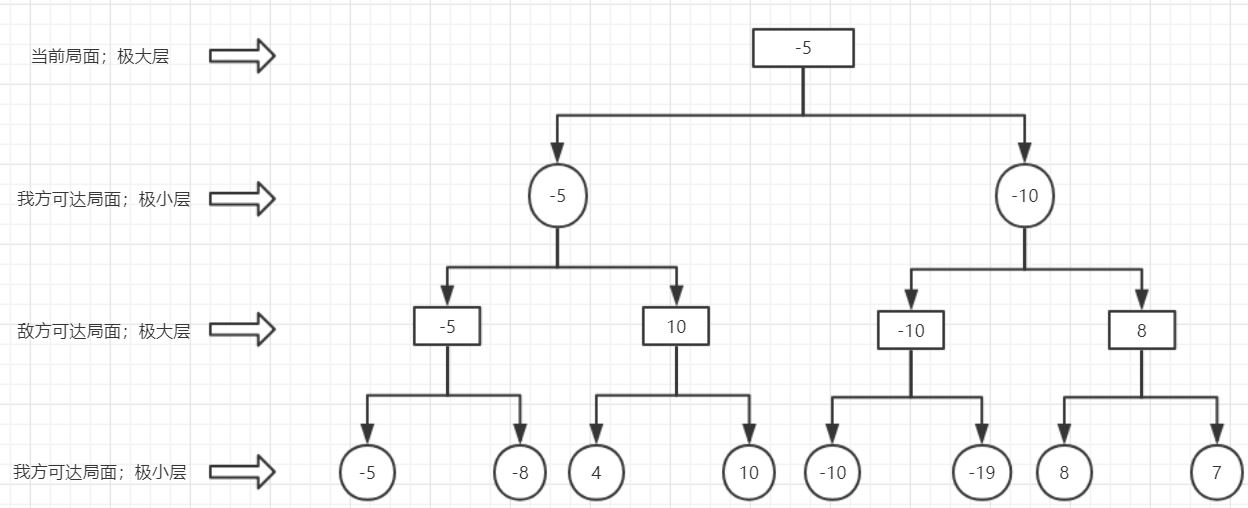
\includegraphics[width=5in]{minmax.jpg}

接下来,考虑一下每一个局面所对应的图节点所需要记录的数据。
\begin{enumerate}
    \item 局面的评估值
    \item 局面所处深度
    \item 生成的所有下一步局面,因为当前局面的评估值由这些局面计算得到
    \item 所走棋子的移动位置,这样才能知晓选择局面是如何到达
\end{enumerate}

那么算法流程如下图:\\
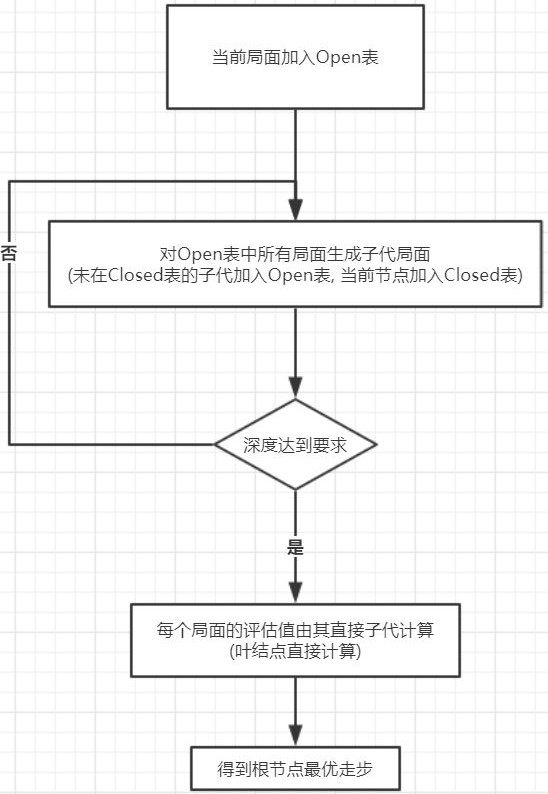
\includegraphics[width=5in]{minmaxAlgorithm.jpg}

具体代码见 \underline{\href{https://github.com/xwy27/ArtificialIntelligenceProjects/blob/master/AI_Web/static/js/ChineseChess/AI.js}{AI.js}},内附详细注释。

\subsection{人机对战-alpha-beta剪枝}

alpha-beta剪枝是对极大极小值搜索的优化。由于极大极小值搜索是遍历所有节点,是穷搜的算法,所以可能会使得搜索宽度过宽而搜索无用节点,导致浪费资源。
这里的剪枝,就是在遇见节点值可被判定无用时,放弃对当前节点后续子代的搜索。那么在极大极小值搜索中,什么时候可以判定放弃搜索呢?
首先,明确一个事实:对于一个极小层节点的评估值b,搜索其子节点时,可以同时更新b值。如一个子节点评估值为5,极小层节点评估值最大为5,因为当前节点会选择最小的。同理,一个极大层节点的评估值a可以同时被评估。
来看两个情况,说明何时放弃搜索:
\begin{enumerate}
    \item 已知当前层为极小层,评估值设为b,其父节点为极大层,评估值设为a,且a最小为10。在搜索当前节点的第一个子节点时,其评估值为5,那么当前节点值最大为5,而a就不可能搜索这个节点的后续节点了,因为前面有10可以选择。
    \item 已知当前层为极大层,评估值设为a,其父节点为极小层,评估值设为b,且b最大为1。在搜索当前节点的第一个子节点时,其评估值为5,那么当前节点值最小为5,而b就不可能搜索这个节点的后续节点了,因为前面有1可以选择。
\end{enumerate}

和极大极小值搜索给出例子对应的alpha-beta剪枝例子如下:\\
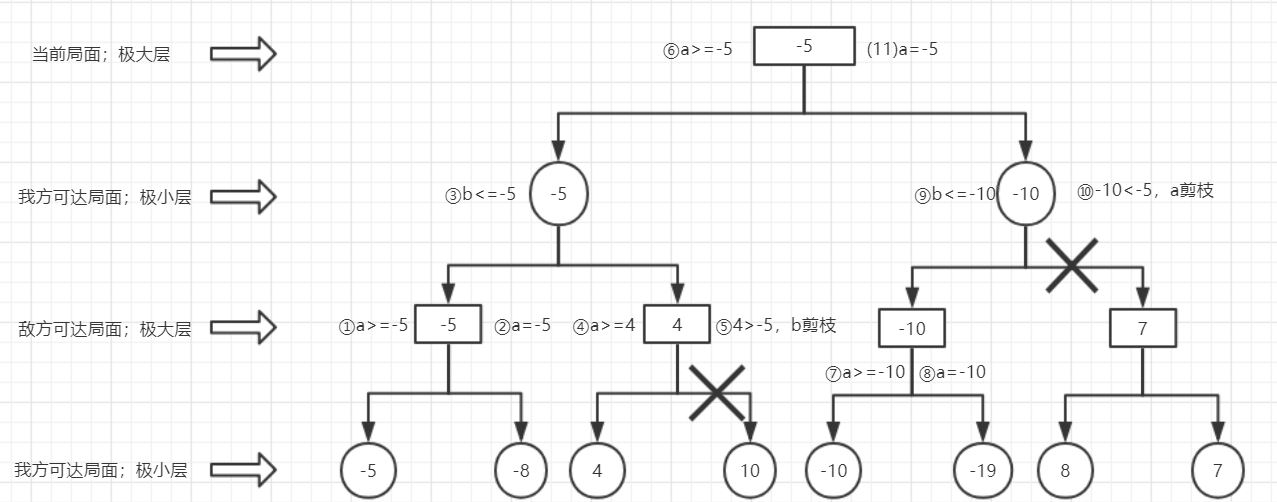
\includegraphics[width=5in]{alphaBeta.jpg}

对应的算法代码,采取了递归实现,因为每一个父节点的值,需要传递给子节点,以作剪枝判断。具体代码见 \underline{\href{https://github.com/xwy27/ArtificialIntelligenceProjects/blob/master/AI_Web/static/js/ChineseChess/AI.js}{AI.js}},内附详细注释。

\section{实验结果与测试}
\begin{enumerate}
    \item 完成极大极小值搜索后,由于属于穷搜算法,搜索深度只可达两层。本人与其对战,其智能程度不足
    \item 更改为alpha-beta剪枝后,搜索深度可达4层。本人与其对战,胜负各半;两位舍友与搜索深度为2层的剪枝AI对战,舍友战绩三负一平
\end{enumerate}

\begin{thebibliography}{}
\bibitem{royhoo} http://www.cnblogs.com/royhoo/p/6425658.html
\end{thebibliography}

\end{document}